\documentclass[a4paper,oneside, draft]{memoir}
\usepackage[T1]{fontenc}
\usepackage[utf8]{inputenc}
\usepackage[english]{babel}

% bedre orddeling Gør at der som minimum skal blive to tegn på linien ved
% orddeling og minimum flyttes to tegn ned på næste linie. Desværre er værdien
% anvendt af babel »12«, hvilket kan give orddelingen »h-vor«.
\renewcommand{\englishhyphenmins}{22} 

\usepackage{colortbl}  % Bruges til at farve celler, rækker mv. i tabeller
\usepackage{pdflscape} % Gør landscape-environmentet tilgængeligt
\usepackage{fixme}     % Indsæt "fixme" noter i drafts.
\usepackage{hyperref}  % Indsæter links (interne og eksterne) i PDF
\usepackage{graphicx}

\renewcommand{\ttdefault}{pcr} % Bedre typewriter font
%\usepackage[sc]{mathpazo}     % Palatino font
\renewcommand{\rmdefault}{ugm} % Garamond
%\usepackage[garamond]{mathdesign}

%\overfullrule=5pt
%\setsecnumdepth{part}
\setcounter{secnumdepth}{-1} % Sæt overskriftsnummereringsdybde. Disable = -1.

\newcommand{\EDSL}{EDSL (Embedded Domain Specific Language) \renewcommand{\EDSL}{ EDSL }}

\title{Controlling embedded devices with funktional reactive programming}

\author{Martin Dybdal (dybber@dybber.dk), \\
Jesper Reenberg (jesper.reenberg@gmail.com) \\ og
Troels Henriksen (athas@sigkill.dk)}

\date{\today}
\pagestyle{plain}



\begin{document}
\maketitle

\begin{abstract}
  Robots are conventionally programmed in low-level imperative
  languages with no concepts like events, synchronicity or any of the
  advantages found in functional programming languages (like pattern
  matching). Reactive programming languages embedded in Haskell, like
  Frob \cite{frob99} and Yampa \cite{arrowsrobotsfrp02}, has been
  suggested for robot programming, but they require a complete Haskell
  runtime system, which is to large to fit on more
  resource-constrained devices. We tie these two ends together,
  creating a highly declarative language for robot programming using a
  staged-compilation strategy like the one found in Flask
  \cite{flask08}, that makes it possible to run programs on devices
  with few resources. In the creation we've used the Flask-codebase as
  a starting point and huge parts of the code is left unchanged.
\end{abstract}


\section{Disposition}
\begin{itemize}
\item Abstract

\item Preface
  \begin{itemize}
  \item Brief intro to robot programming
    \begin{itemize}
     \item Sensors and Actuators
    \end{itemize}
  \item Brief Arduino introduction
  \item Brief Flask introduction
    \begin{itemize}
     \item The staged compilation strategy
    \end{itemize}
  \end{itemize}

\item Previous Work
  \begin{itemize}
  \item Frob
  \item Esterel
    (http://www.softwaresafety.net/Esterel.org/esterel.html)
  \item Lustre \cite{lustre91}
  \item Flask
  \end{itemize}

\item "`Our system"'
  \begin{itemize}
  \item Staged compilation
  \item Dataflows
  \item Node representation
  \item Devices
  \item Interrupts
  \item Events
  \end{itemize}

\item Example programs

\item Conclusions

\item Bibliography

\item Appendixes
  \begin{itemize}
  \item A Flask tour
  \item Small guide to Arduino and electronics
  \end{itemize}
\end{itemize}  

\bibliographystyle{plain}
\bibliography{rapport}

\appendix

\chapter{Small guide to Arduino and electronics}

\begin{quotation}
  Arduino is an open-source electronics prototyping platform based on
  flexible, easy-to-use hardware and software. It's intended for
  artists, designers, hobbyists, and anyone interested in creating
  interactive objects or environments.

  Arduino can sense the environment by receiving input from a variety
  of sensors and can affect its surroundings by controlling lights,
  motors, and other actuators. The microcontroller on the board is
  programmed using the Arduino programming language (based on Wiring)
  and the Arduino development environment (based on
  Processing). Arduino projects can be stand-alone or they can
  communicate with software on running on a computer (e.g. Flash,
  Processing, MaxMSP).
\end{quotation}

\fixme{This is citet from Arduinos homepage the 28. of April 2009 at 15:16}

\fixme{<<Image of our Duemilanove>>}

There are different kinds of Arduino boards. All are based on
different ATmega* processors from Atmel. The older boards used serial
communication while the newer ones are connected to the computer
through a USB cable, but still using the same serial communication
protocol (i.e. serial through USB). The USB cable also serves as a
power supply.


We will describe the Arduino Duemilanove board we have used, in the
sections that follow, but most information will apply to
the other Arduino boards as well.

\section{Pins}
The Arduino board can connect to several external components through
diverse input and output pins. The pins are split in three sections on
the board \textit{power}, \textit{analog in} and
\textit{digital}. Before any IO can happen on a pin, it's mode must be
set. The mode of a pin defines if it is to be used to read input or
write output. The mode is set by the function \texttt{void pinMode(int
  pinnumber, int mode)} where \textit{pinnumber} is a number between
0-5 for analog and 0-13 for digital and \textit{mode} is either
\texttt{OUTPUT} or \texttt{INPUT}.

\subsection{Power pins}
\begin{itemize}
\item Reset: Resets the board when connected to ground. \fixme{tror jeg i
    hvert fald..}
\item 3V3: Constant 3,3v output
\item 5v: Constant 5v output
\item Gnd: Ground
\item Gnd: Ground
\item Vin: External power supply connection (9v recomented)
\end{itemize}

\subsection{Digital pins}
There are 14 digital input and output pins from which 6 of them can be
used to generate analog output by PWM (Pulse Width Modulation). It's
possible to read a boolean value \texttt{HIGH} and \texttt{LOW} by the
following function \texttt{bool digitalRead(int pinnumber)} where
pinnumber is a number between 0 and 13. It's possible to write a
boolean value by the following function \texttt{void digitalWrite(int
  pinnumber, int value)} where pinnumber is a number between 0 and 13
and value is either \texttt{HIGH} or \texttt{LOW}.

\subsection{Analog input}
There are 6 analog input pins. It's possible to read a voltage level
from each of them using the function \texttt{int analogRead(int
  pinnumber)} where \textit{pinnumber} is a number between 0 and 5
indicating which pin to read from. The result is given as an integer
in the range from 0 to 1023. It's possible to write a voltage level
(PWM wave, explained below) by the following function \texttt{void
  analogWrite(int pinnumber, int value)} where \textit{pinnumber} is
one of (3,5,6,9,10,11) which is located among the 14 digital pins and
\textit{value} is an integer in the range from 0 to 255. The reason
why the 6 analog output pins is located among the digital IO pins is
that the platform uses PWM to generate the desired voltage level.

\subsubsection{PWM}

\begin{quotation}
  Pulse Width Modulation, or PWM, is a technique for getting analog
  results with digital means. Digital control is used to create a
  square wave, a signal switched between on and off. This on-off
  pattern can simulate voltages in between full on (5 Volts) and off
  (0 Volts) by changing the portion of the time the signal spends on
  versus the time that the signal spends off. The duration of "on
  time" is called the pulse width. To get varying analog values, you
  change, or modulate, that pulse width. If you repeat this on-off
  pattern fast enough with an LED for example, the result is as if the
  signal is a steady voltage between 0 and 5v controlling the
  brightness of the LED.

  In the graphic below, the green lines represent a regular time
  period. This duration or period is the inverse of the PWM
  frequency. In other words, with Arduino's PWM frequency at about
  500Hz, the green lines would measure 2 milliseconds each. A call to
  analogWrite() is on a scale of 0 - 255, such that analogWrite(255)
  requests a 100\% duty cycle (always on), and analogWrite(127) is a
  50\% duty cycle (on half the time) for example.

  
  \begin{figure}[h!]
    \centering
    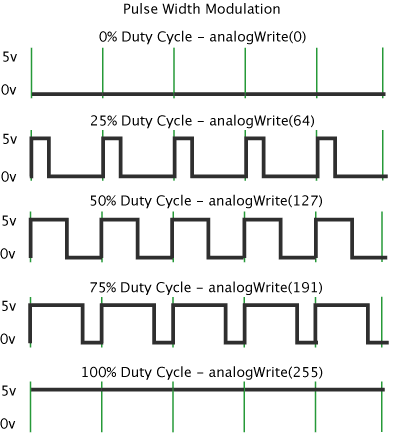
\includegraphics[scale=0.8]{images/pwm}

    \caption{How 0\%, 25\%, 50\%, 75\% and 100\% PWM is messured by a
      osciloscope. Where Each vertical green line indicates the duty
      cycle}
    \label{fig:pwm}
  \end{figure}

  \fixme{Better figure text and figure should be non-floating. Jesper
    has a solution to this in his old Graphics report}

  Once you get this example running, grab your Arduino and shake it
  back and forth. What you are doing here is essentially mapping time
  across the space. To our eyes, the movement blurs each LED blink
  into a line. As the LED fades in and out, those little lines will
  grow and shrink in length. Now you are seeing the pulse width.
\end{quotation}
\fixme{taken from \url{http://www.arduino.cc/en/Tutorial/PWM} on the
  28. of April at 17:14}

\section{Timer Interrupts}

\fixme{fix text to support new heading: timer interrupts}

The ATmega168/ATmega328 processors has three different hardware
timers. One of them (timer 1) is used by Arduino software to provide a
\texttt{millis()} function that gives us the amount of milliseconds
since the timer started and a \texttt{delay} function that actively
holds the processor occupied for a given time period. Timer 0 and 2
uses 8 bit registers and timer 1 uses a 16 bit register. This
effectively means that timer 0 and 2 can't count to more than 255
whereas timer 1 can count to 65535. The registers is incremented at
the speed of the processor, in this case 16MHz, divided by a prescale
factor which can be either of 1,2,4,8,16,32,64,128 or 256. The three
timers modes of operation is \texttt{Normal}, \texttt{CTC}(Clear Timer
on Compare match), \texttt{Fast PWM}, \texttt{Phase Correct PWM} where
\texttt{Normal} and \texttt{CTC} are the ones of
interrest: 



\begin{description}
\item[\texttt{Normal}] mode counts from a optionally specified counter
  value (initially default set to 0) and increments until it reaches
  the maximum value 255 where it overruns, restarts from 0, the
  interrupt is triggered and incrementation of the counter
  restarts.

\item[\texttt{CTC}] mode has a predefined top value and optionally
  specified counter value (initially default set to 0). When the
  counter reaches the defined top value it is cleared to 0, the
  interrupt is triggered and incrementation of the counter
  restarts. This gives better resolution of the counter and thus more
  flexibility than the \texttt{Normal} mode.
\end{description}

The modes of operation is described in detail in the processors
datasheet, section 12.7 ``Modes of Operation''.

\fixme{Interference problems with the PWM output pins.}  
\fixme{Better explanation about prescale modes}

\section{External Interrupts}

Essentialy all the pins on the Arduino board supports external
interrupts, though only digital pins 2 and 3 is supported directley by
the Arduino code via the function \texttt{void attachInterrupt(int
  interruptpin, void (* userfunc)(void), int mode)} where
\textit{interruptpin} is either 0 or 1, \textit{userfunc} is the user
function to call when the interrupt triggers and \textit{mode} is one
of \texttt{LOW}, \texttt{CHANGE}, \texttt{RISING} or
\texttt{FALLING}. The \textit{mode} property is special for these two
external interrupt pins, as the other pins only support the
\texttt{CHANGE} mode. The full descriptions of the modes is in the
datasheet of the processor section 10.2.1 ``EICRA - External Interrupt
Control Register A''. To set up external interrupts on the other pins
the user ckiick has added an useable header file to the Arduino
playground\footnote{\url{http://www.arduino.cc/playground/Main/PcInt}
  taken tuesday the 28. of April 2009 at 16:45} also containing an
example of how it works. This headerfile defines a function
\texttt{void PCattachInterrupt(int interruptpin, void (*
  userfunc)(void), int mode)} where the only difference is that the
\textit{mode} property only supports \texttt{CHANGE}.


\section{Electronics}
\fixme{Maybe a little refresher on electronics (e.g. how each
  component are drawn in a diagram, if we are going to use diagrams in
  the article). }

\end{document}
